%& C:\Users\RANGAR~1\AppData\Roaming\TikzEdt\TikzEdt\023~1.0\TEMP_H~1
\begin{document}
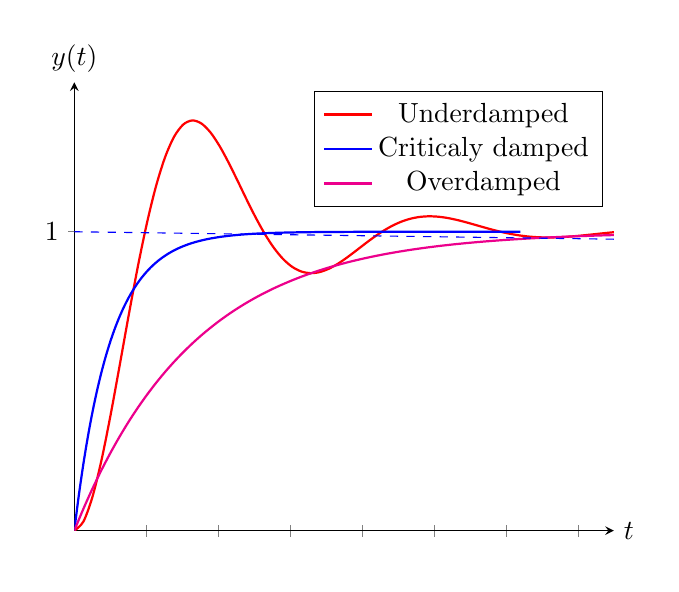
\begin{tikzpicture}
% https://tex.stackexchange.com/questions/312523/step-response-in-tikz
\begin{axis}[
        axis lines=middle,
        xmin=0, xmax=15,
        ymin=0, ymax=1.5,
        xlabel=$t$,
        ylabel={$y(t)$},
        xlabel style={at=(current axis.right of origin), anchor=west},
        ylabel style={at=(current axis.above origin), anchor=south},
        %xtick={0, 0.4726, 1.79398, 1.96605, 3.2236, 11.0855},
        %xticklabels={$0$, $t_{r_1}$, $t_{r_1}$, $t_r$, $t_p$, $t_s$},
        xticklabels = none,
        %ytick={0, 0.1, 0.9, 1, 1.3714},
        %yticklabels={$0$, $0.1$, $0.9$, $1$, $M_p$}
        ytick = {0,1},
        yticklabels = {0,1},
    ]
    \addplot[smooth, 
             red,
             thick,
             mark=none,
             domain=0:25,
             samples=100]
    {1-exp(-0.3*x)*(cos(deg(sqrt(1-0.3^2)*x))+0.3/(sqrt(1-0.3^2))*sin(deg(sqrt(1-0.3^2)*x)))};
    
    \addplot[smooth, 
             blue,
             thick,
             mark=none,
             domain=0:12.4,
             samples=100] {1-exp(-1*x)};
             
     \addplot[smooth, 
             magenta,
             thick,
             mark=none,
             domain=0:25,
             samples=100] {1-exp(-0.3*x)};
    %
%     \addplot[black, dotted] coordinates{(0.4726,0.1)} -- (axis cs:0,0.1);
%     \addplot[black, dotted] coordinates{(0.4726,0.1)} -- (axis cs:0.4726,0);
%     %
%     \addplot[black, dotted] coordinates{(1.79398,0.9)} -- (axis cs:0,0.9);
%     \addplot[black, dotted] coordinates{(1.79398,0.9)} -- (axis cs:1.79398,0);
%     %
%     \addplot[black, dotted] coordinates{(1.96605,1)} -- (axis cs:1.96605,0);
%     %
%     \addplot[black, dotted] coordinates{(3.2236,1.3714)} -- (axis cs:0,1.3714);
%     \addplot[black, dotted] coordinates{(3.2236,1.3714)} -- (axis cs:3.2236,0);
%     %
%     \addplot[black, dotted] coordinates{(11.0855,1.025)} -- (axis cs:11.0855,0);
%     %
%     \addplot[black, thick] coordinates{(15,0.9872)} -- (axis cs:12.4,0.9872);
%     %
%     \addplot[black, dashed] coordinates{(15,1)} -- (axis cs:0,1);
%     %
	 \addplot[blue, dashed] coordinates{(15,0.975)} -- (axis cs:0,1);
%     \addplot[blue, dashed] coordinates{(15,1.025)} -- (axis cs:0,1.025);

    %\coordinate (a) at (axis cs:0,0);
    %\coordinate (b) at (axis cs:1.79398,0);
	\legend{Underdamped,Criticaly damped, Overdamped},
    \end{axis}

    %\draw [shorten <=1mm,shorten >=1mm] (a) -- ++(0,-1cm) coordinate (aa);
    %\draw (b) -- ++(0,-1cm) coordinate (bb);
    %\draw [|<->|] (aa) -- (bb) node [midway,fill=white] {$t_r$};

    
\usetikzlibrary{calc}
\pgftransformreset
\node[inner sep=0pt,outer sep=0pt,minimum size=0pt,line width=0pt,text width=0pt,text height=0pt] at (current bounding box) {};
%add border to avoid cropping by pdflibnet
\foreach \border in {0.1}
  \useasboundingbox (current bounding box.south west)+(-\border,-\border) rectangle (current bounding box.north east)+(\border,\border);
\newwrite\metadatafile
\immediate\openout\metadatafile=\jobname_BB.txt
\path
  let
    \p1=(current bounding box.south west),
    \p2=(current bounding box.north east)
  in
  node[inner sep=0pt,outer sep=0pt,minimum size=0pt,line width=0pt,text width=0pt,text height=0pt,draw=white] at (current bounding box) {
\immediate\write\metadatafile{\p1,\p2}
};
\immediate\closeout\metadatafile
\end{tikzpicture}

\end{document}
\end{document}
